\documentclass[12pt]{article}

\usepackage[utf8]{inputenc}
\usepackage{listings}
\usepackage{graphicx}
\usepackage{float}
\usepackage{geometry}

\usepackage{parskip}
\setlength{\parskip}{1.0\baselineskip plus2pt minus2pt}

\addtolength{\topmargin}{-50pt}
\addtolength{\textheight}{130pt}
\addtolength{\textwidth}{95pt}
\addtolength{\oddsidemargin}{-45pt}

\title{Simulação e Computação Científica - Trabalho 1}
\author{David Gomes (2013136061), Nuno Gonçalves (2012139146), Marta Mercier (2013136742)}
\date{Março 2015}

\begin{document}
\maketitle

\section*{Introdução}
O primeiro trabalho de Simulação e Computação Científica consiste num ecossistema
descrito por uma grelha bidimensional com vegetação, habitado por lobos e ovelhas.

Ao simularmos o ambiente, implementado em Java, detetámos que tanto os lobos como
as ovelhas morriam prematuramente (os lobos extinguiam-se depois de mais ou menos
700 iterações). Assim, encontrámos valores mais apropriados para a simulação, de
forma a que este seja um ecossistema estável, ou seja, para que haja sempre lobos, ovelhas e vegetação durante as 5000 unidades de tempo.

Apresentamos, de seguida, os diferentes resultados obtidos de acordo com os dados do
enunciado e de acordo com os novos valores que encontrámos.

\section*{Resultados}
\subsection{Valores do Enunciado}

\begin{figure}[H]
  \centering
  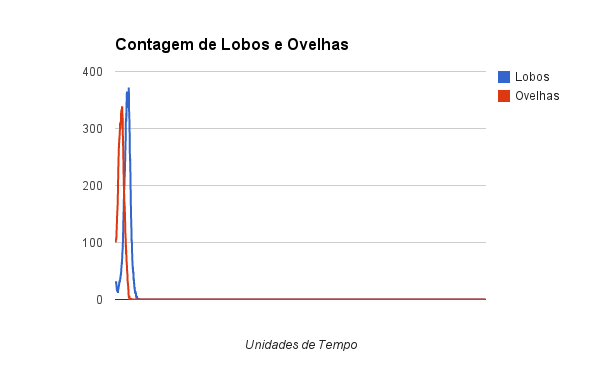
\includegraphics[width=0.75\textwidth]{ovelhaslobos1}
  \caption{Distribuição de Lobos e Ovelhas}
\end{figure}

Podemos observar neste gráfico que, utilizando os dados do enunciado, ao fim de, aproximadamente, 700 unidades de tempo todas as ovelhas morrem (morte esta que pode ser causada por vários factores: a predação dos lobos, o facto de não encontrarem vegetação ou uma pequena taxa de reprodução) o que causa também a morte dos lobos, que acabam por ficar sem alimento.

\begin{figure}[H]
  \centering
  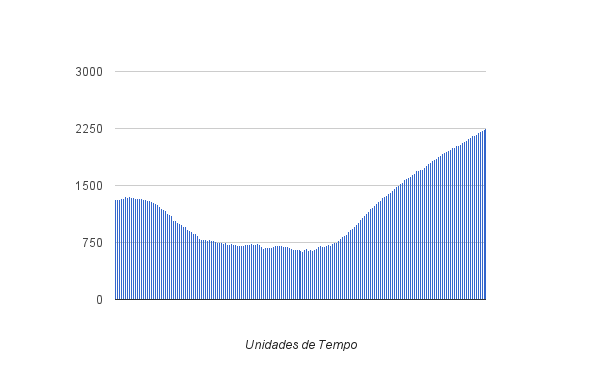
\includegraphics[width=0.75\textwidth]{vegetacao1}
  \caption{Evolução da Vegetação, em unidades}
\end{figure}

Analisando este gráfico podemos observar que, com o aumento do número de ovelhas, há um decréscimo de vegetação e após a morte dos animais esta cresce continuamente.

\subsection{Valores Alterados}

\begin{figure}[H]
  \centering
  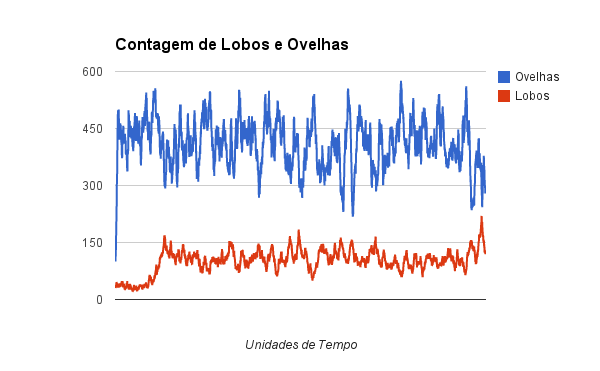
\includegraphics[width=0.75\textwidth]{ovelhaslobos2}
  \caption{Distribuição de Lobos e Ovelhas}
\end{figure}

Para obter este resultado, alterámos a probabilidade de reprodução das ovelhas, que aumentamos
de \texttt{0.04} para \texttt{0.10} e a energia ganha pelos lobos ao comer uma ovelha, que
diminuimos de \texttt{20} para \texttt{6}.

Podemos notar, neste gráfico, o rápido crescimento do número de ovelhas nas primeiras iterações
da simulação, uma vez que aumentámos a probabilidade de reprodução destas. Notamos ainda que o número de lobos nunca é muito elevado (nem superior ao número de ovelhas), devido à diminuição da energia ganha quando se alimentam, o que faz com que o tempo de vida de cada lobo seja menor.

\begin{figure}[H]
  \centering
  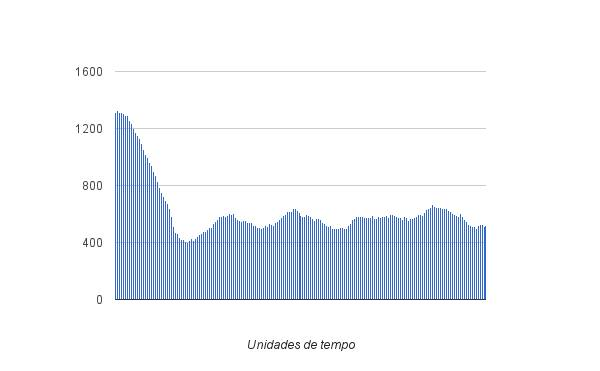
\includegraphics[width=0.75\textwidth]{vegetacao2}
  \caption{Evolução da Vegetação, em unidades}
\end{figure}

Neste caso observamos, inicialmente, um decréscimo acentuado da vegetação, devido ao grande aumento do número de ovelhas. Após os momentos iniciais, a evolução da vegetação estabiliza, mantendo-se dentro dos mesmo valores, aproximadamente.

\section*{Análise de Resultados e Conclusão}

Podemos concluir, comparando os gráficos da evolução da vegetação entre os dois
\textit{datasets}, que a vegetação é muito mais constante com os valores alterados.
Isto acontece porque o crescimento e decrescimento estável das ovelhas faz com que a vegetação cresça linearmente.

Para além disto, obervamos que, enquanto no primeiro caso há um aumento acentuado de animais seguido de um decréscimo brusco até à sua morte, na segunda situação a quantidade de animais se mantém mais estável desde o início até ao fim da simulação.

Concluímos assim que os novos valores encontrados permitem manter um ecossistema equilibrado, mantendo vegetação, lobos e ovelhas vivos até ao final das 5000 iterações.


\end{document}
